\documentclass[10pt]{beamer}
\usepackage[utf8]{inputenc}
\usepackage{hyperref}
\hypersetup{colorlinks=true,linkbordercolor=blue,linkcolor=white,urlcolor=blue,pdfborderstyle={/S/U/W 1}}

\usepackage[scaled]{helvet}
\usepackage[T1]{fontenc}
\usetheme{Berkeley}
\beamertemplatenavigationsymbolsempty
\setbeamertemplate{headline}{}
\setbeamersize{sidebar width left=1.5cm}
\setbeamerfont{section in sidebar}{size=\fontsize{6}{3.5}\selectfont}
\setbeamerfont{title in sidebar}{size=\fontsize{6}{6}\selectfont}
\title{Create a FoodChain-Lab Workflow}
\date{}

\begin{document}
\maketitle

\section{Topics}
\begin{frame}
\leftskip1em\textbf{Learn}
	\begin{itemize}
      \item to import a FoodChain-Lab template.
      \item to display and configure the delivery network.
      \item to visualize the backward and forward trace for a station.
    \end{itemize}
\end{frame}

\section{1}
\begin{frame}
	\begin{center}
  		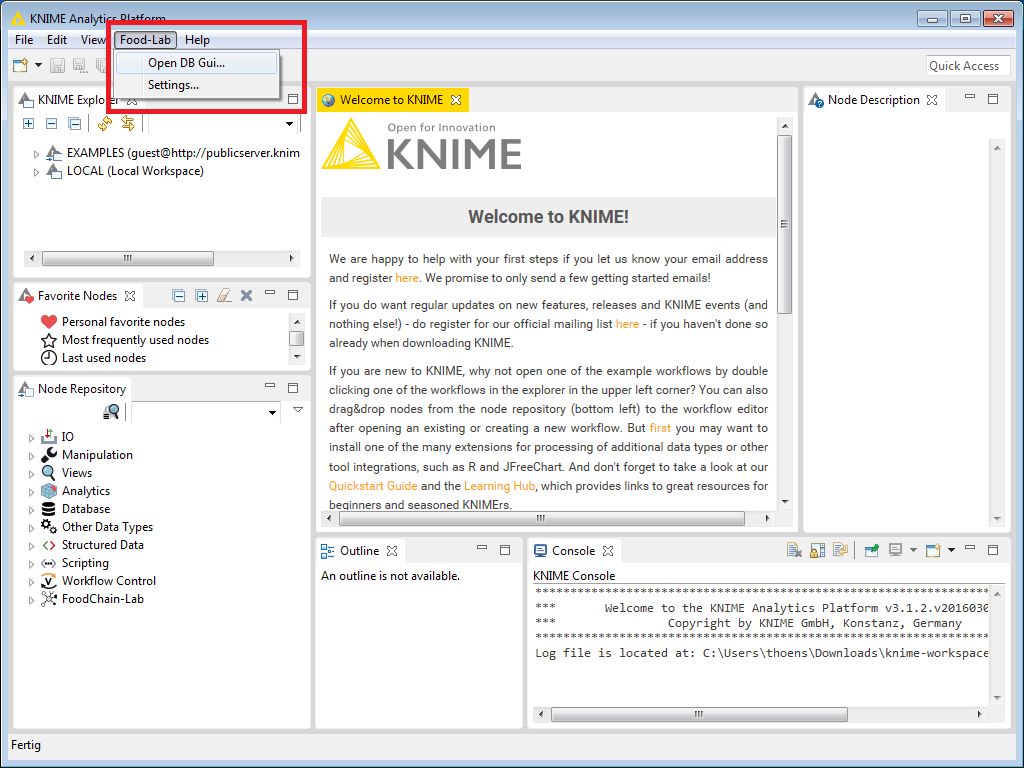
\includegraphics[height=0.6\textheight]{1.png}
	\end{center}
	\begin{itemize}
		\item Select \textbf{Food-Lab} and \textbf{Open DB Gui...} in the menu bar to open the database interface.
	\end{itemize}
\end{frame}

\section{2}
\begin{frame}
	\begin{center}
  		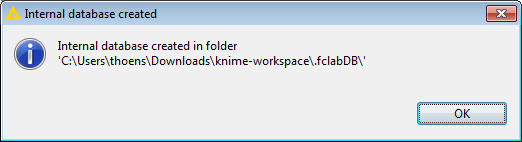
\includegraphics[width=0.9\textwidth]{2.png}
	\end{center}
	\begin{itemize}
		\item If you get a message saying the internal database has been created, click \textbf{OK}. If not, the database has obviously been created before.
	\end{itemize}
\end{frame}

\section{3}
\begin{frame}
	\begin{center}
  		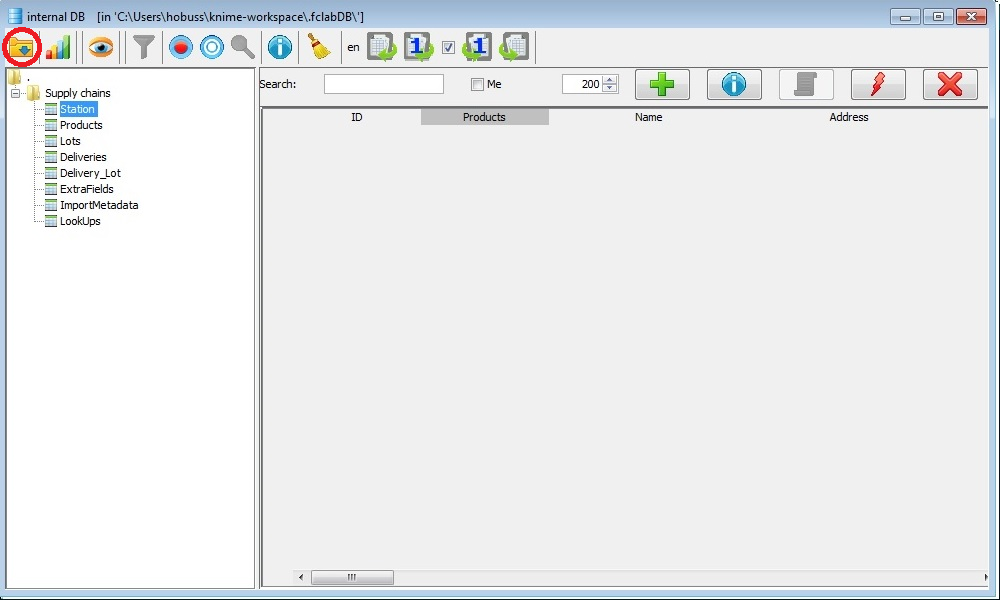
\includegraphics[height=0.6\textheight]{3.png}
	\end{center}
	\begin{itemize}
		\item Download the example file from \textcolor{blue}{\underline{\href{https://github.com/SiLeBAT/BfROpenLabResources/raw/master/GitHubPages/documents/FCL_Create_a_FoodChain-Lab_Workflow/FCL_Examples.xlsx}{``FCL\_Examples.xlsx''}}}.
		\item In the database interface click the \textbf{Table import} button in the upper left corner.
	\end{itemize}
\end{frame}

\section{4}
\begin{frame}
	\begin{center}
  		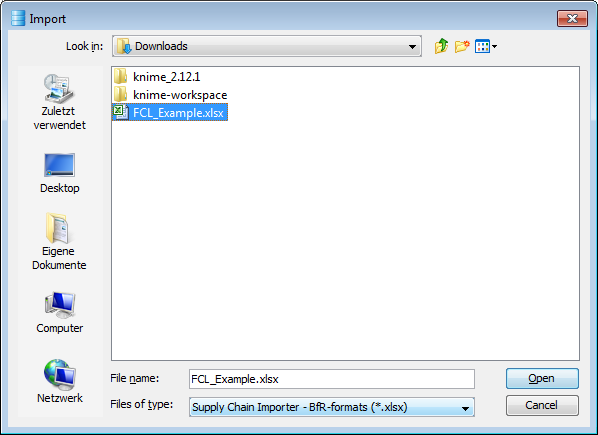
\includegraphics[height=0.6\textheight]{4.png}
	\end{center}
	\begin{itemize}
		\item Now, a file dialog will pop up. FoodChain-Lab data templates (*.xlsx files) can be selected here.
		\item Navigate to the folder with the file ``FCL\_Examples.xlsx'' which you have  downloaded.  Select the file in the dialog and press \textbf{Open}.
	\end{itemize}
\end{frame}

\section{5}
\begin{frame}
	\begin{center}
  		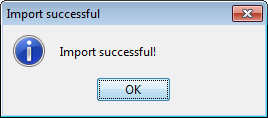
\includegraphics[width=0.5\textwidth]{5.png}
	\end{center}
	\begin{itemize}
		\item If errors or warnings occurred during the import process you would see a dialog after the import is finished.
		\item As no errors ocurred, there is no such dialog and you can click \textbf{OK}.
	\end{itemize}
\end{frame}

\section{6}
\begin{frame}
	\begin{center}
  		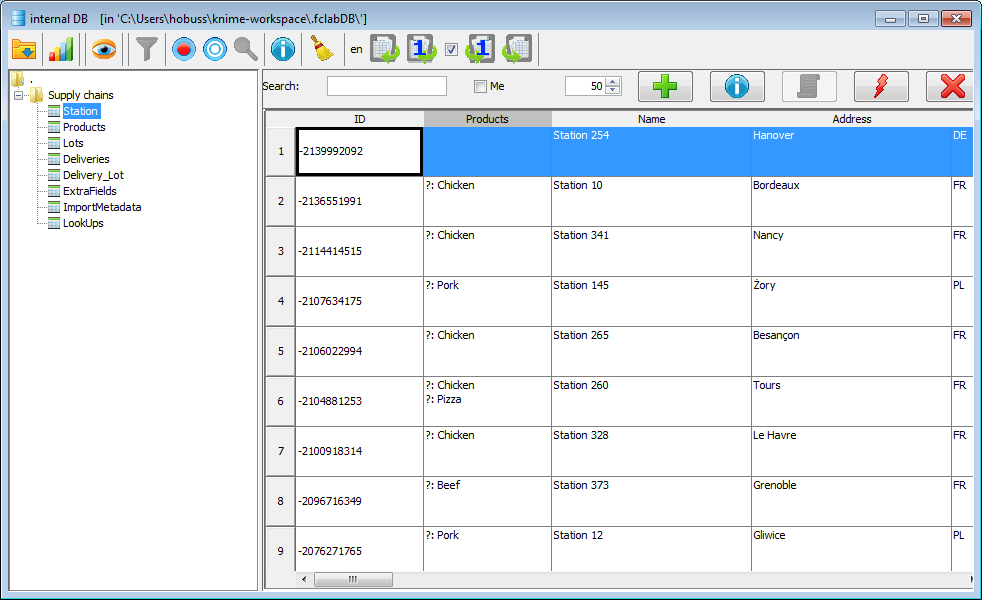
\includegraphics[height=0.6\textheight]{6.png}
	\end{center}
	\begin{itemize}
		\item In the database interface, you can now have a look at the data you have imported.
		\item Close the dialog.
	\end{itemize}
\end{frame}

\section{7}
\begin{frame}
	\begin{center}
  		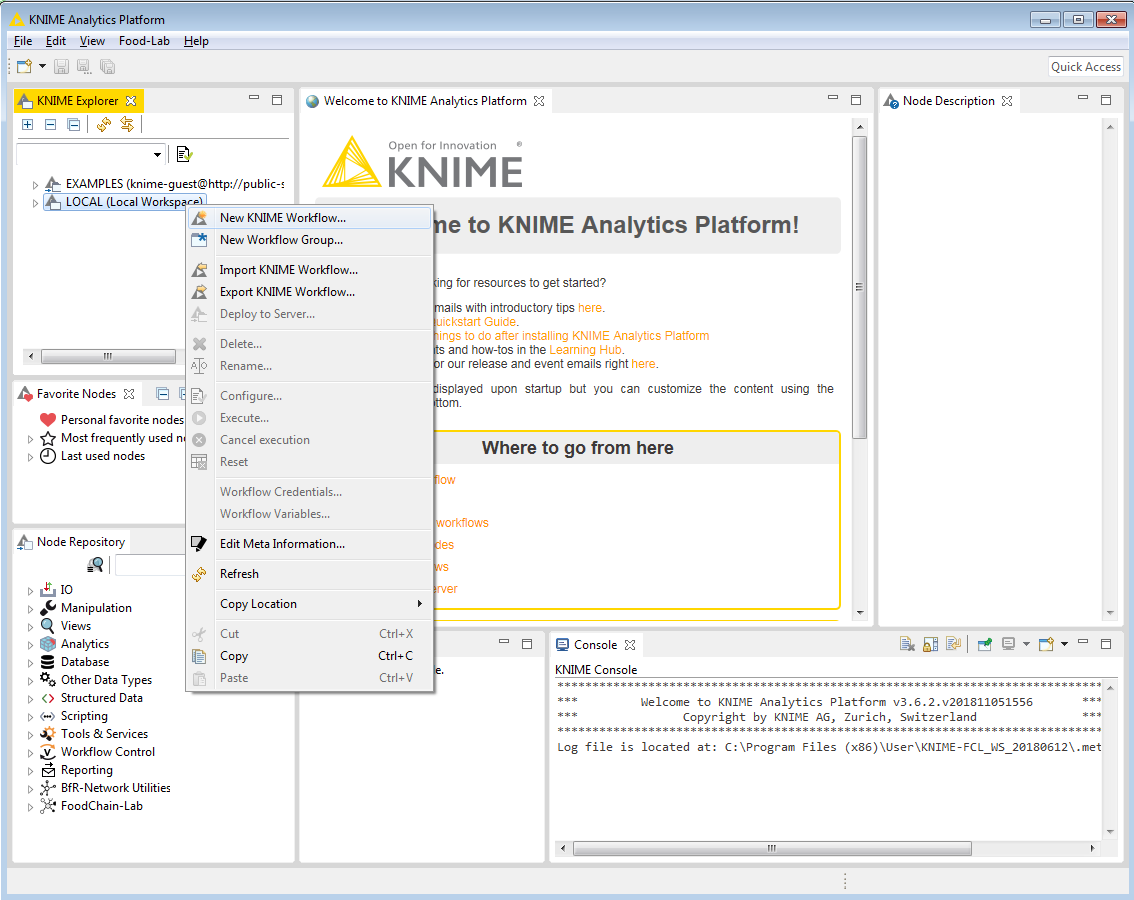
\includegraphics[height=0.6\textheight]{7.png}
	\end{center}
	\begin{itemize}
		\item Now we want to create a workflow, that uses the imported data.
		\item Right click on \textbf{LOCAL} in the \textbf{KNIME Explorer} and select \textbf{New KNIME Workflow...}
	\end{itemize}
\end{frame}

\section{8}
\begin{frame}
	\begin{center}
  		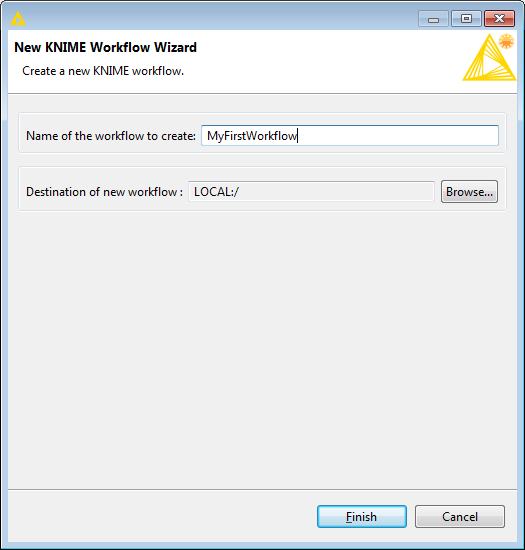
\includegraphics[height=0.6\textheight]{8.png}
	\end{center}
	\begin{itemize}
		\item In the dialog you need to give the workflow a name. How about ``MyFirstWorkflow''?
		\item Click \textbf{Finish}.
	\end{itemize}
\end{frame}

\section{9}
\begin{frame}
	\begin{center}
  		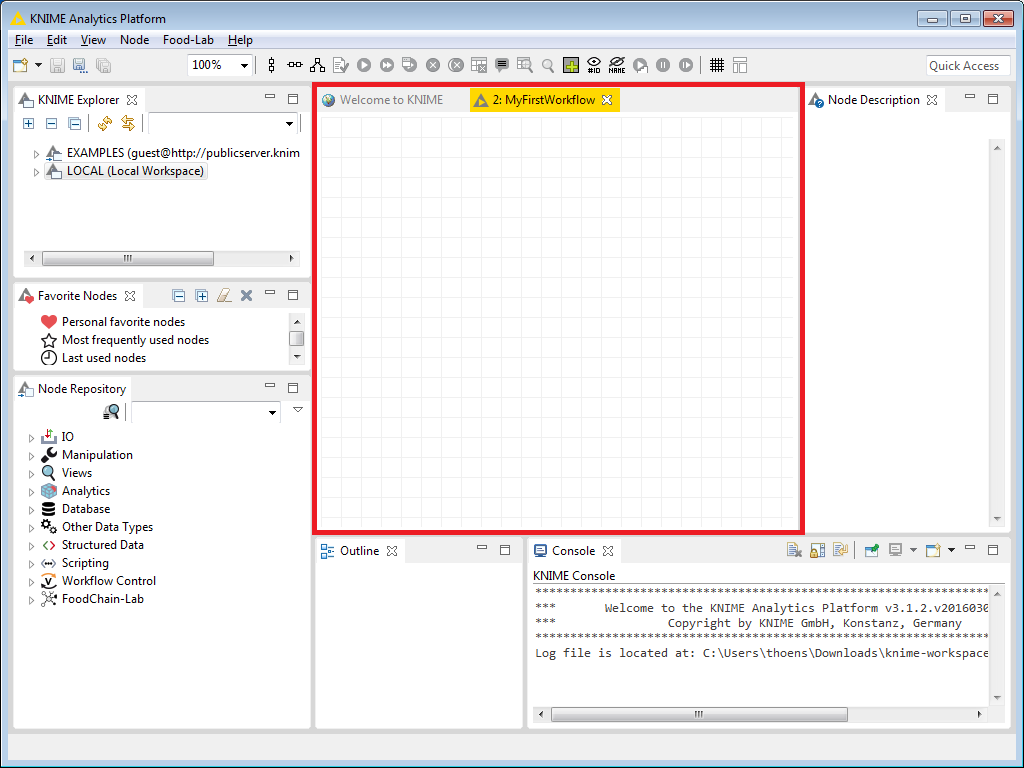
\includegraphics[height=0.6\textheight]{9.png}
	\end{center}
	\begin{itemize}
		\item The created empty workflow will be shown in the editor in the center. Here you can add nodes to build your workflow.
	\end{itemize}
\end{frame}

\section{10}
\begin{frame}
	\begin{center}
  		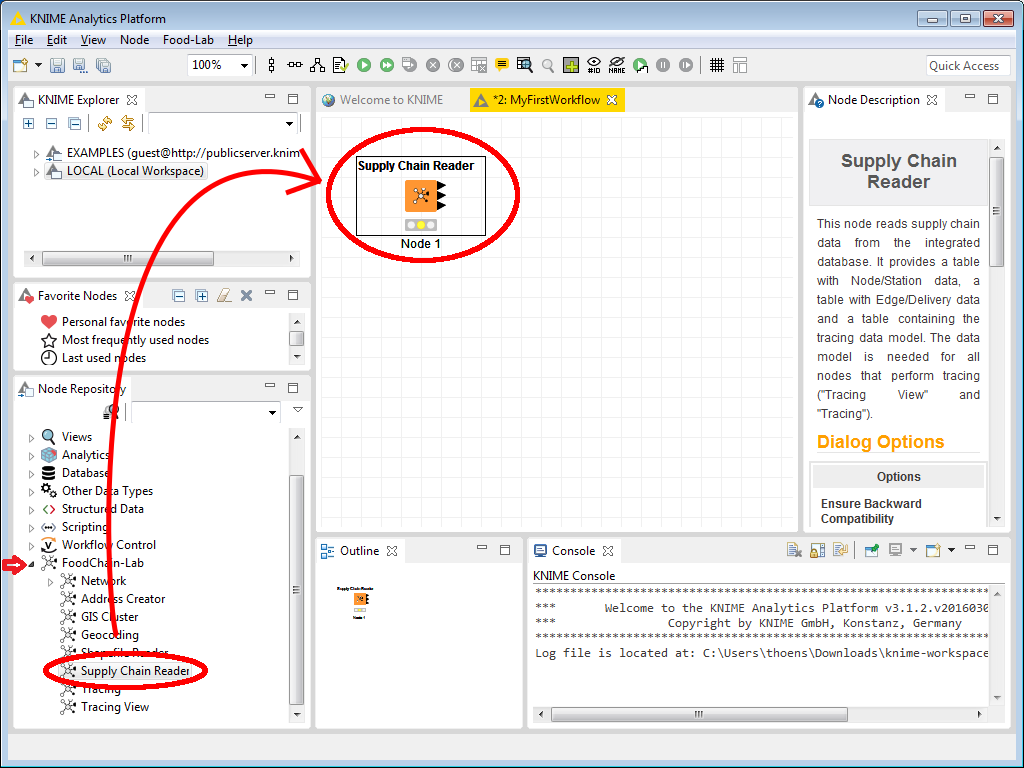
\includegraphics[height=0.6\textheight]{10.png}
	\end{center}
	\begin{itemize}
		\item Now we need FoodChain-Lab nodes. You can find them in the \textbf{Node Repository} on the left. Click on the small arrow on the left of ``FoodChain-Lab'' to show all FoodChain-Lab nodes.
		\item Drag the \textbf{Supply Chain Reader} from the \textbf{Node Repository} into your empty workflow.
	\end{itemize}
\end{frame}

\section{11}
\begin{frame}
	\begin{center}
  		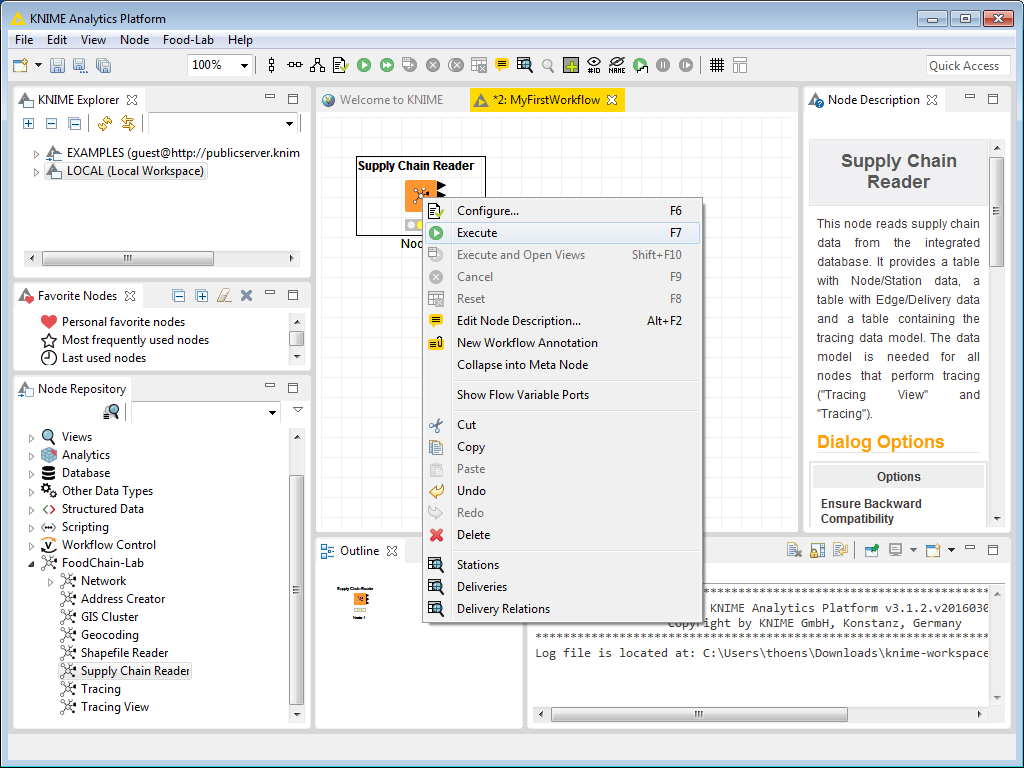
\includegraphics[height=0.6\textheight]{11.png}
	\end{center}
	\begin{itemize}
		\item We do not need to configure the \textbf{Supply Chain Reader}.
		\item Right click on it and select \textbf{Execute}.
	\end{itemize}
\end{frame}

\section{12}
\begin{frame}
	\begin{center}
  		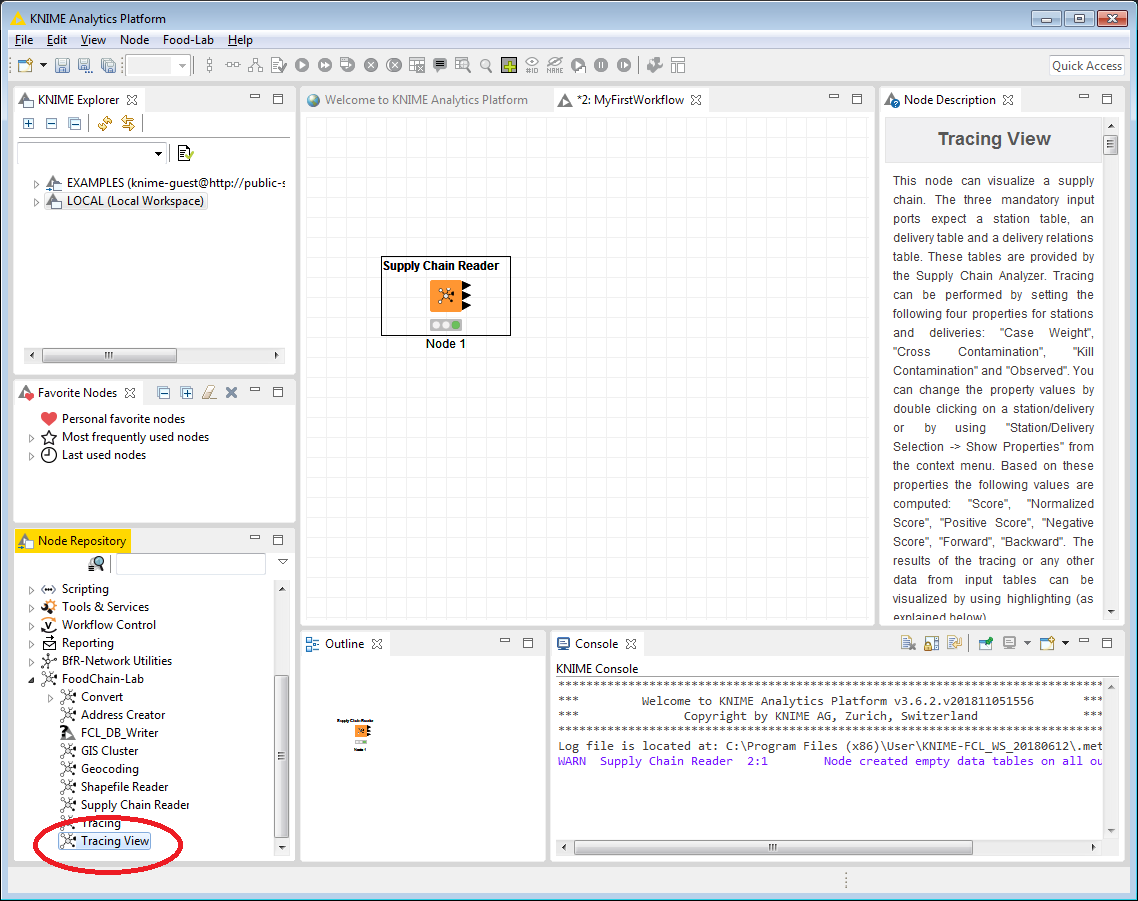
\includegraphics[height=0.6\textheight]{12.png}
	\end{center}
	\begin{itemize}
		\item The \textbf{Supply Chain Reader} has now read all data from the internal database.
		\item Select the \textbf{Supply Chain Reader} in the workflow (so that a rectangle is drawn around it), then double click on the \textbf{Tracing View} node in the \textbf{Node Repository}.
	\end{itemize}
\end{frame}

\section{13}
\begin{frame}
	\begin{center}
  		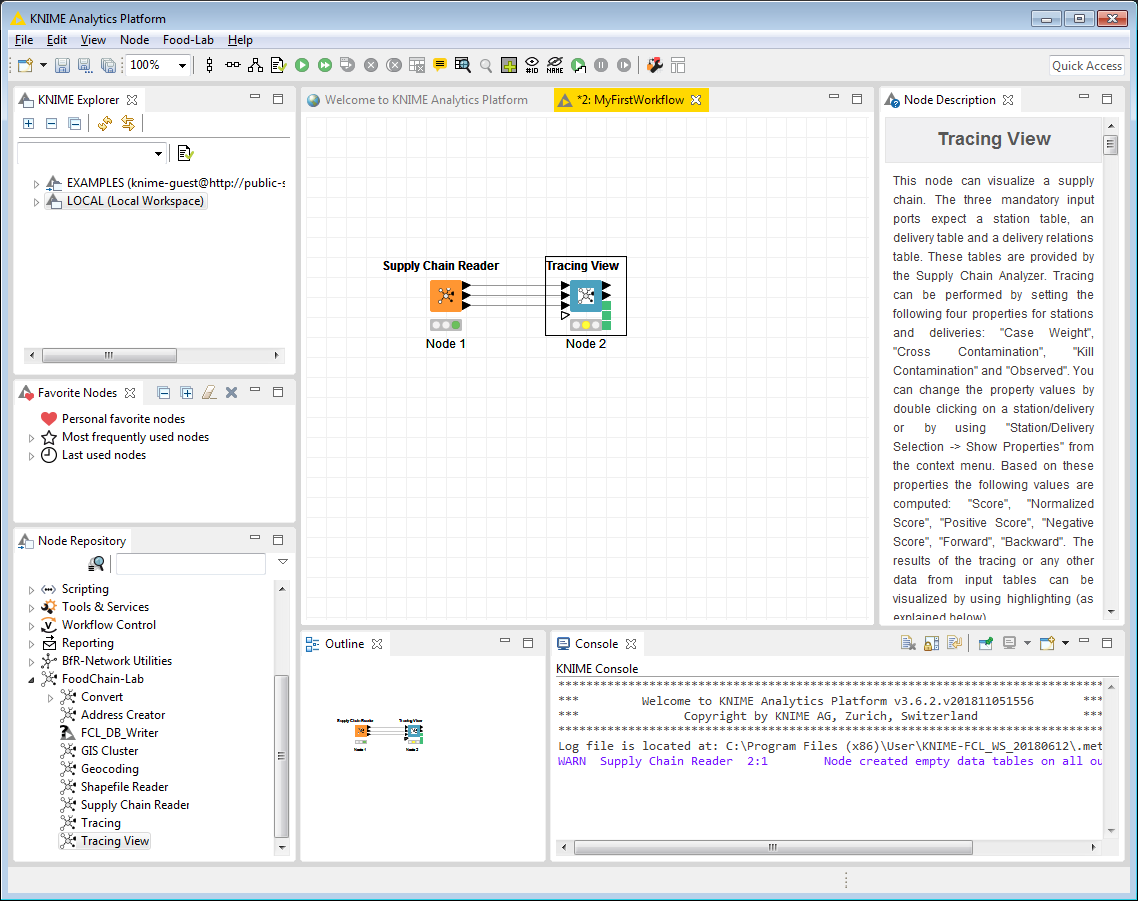
\includegraphics[height=0.6\textheight]{13.png}
	\end{center}
	\begin{itemize}
		\item The \textbf{Tracing View} node should show up in the workflow and its three input ports should be automatically connected to the \textbf{Supply Chain Reader}. This is the fastes way to attach one node to another.
	\end{itemize}
\end{frame}

\section{14}
\begin{frame}
	\begin{center}
  		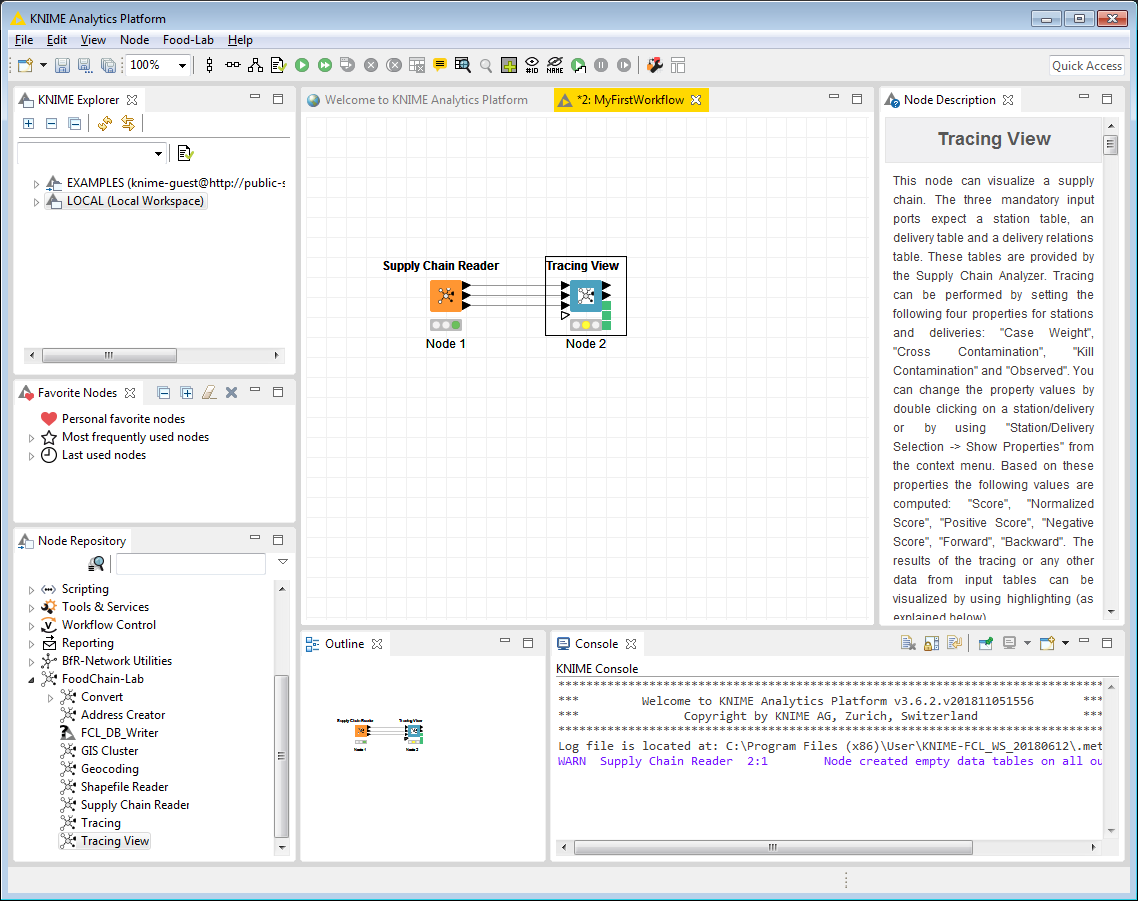
\includegraphics[height=0.6\textheight]{13.png}
	\end{center}
	\begin{itemize}
		\item Another option would be to drag the \textbf{Tracing View} node from the \textbf{Node Repository} into the editor. Then left click on the upper output port of the \textbf{Supply Chain Reader} (black arrow), keep pressing the left mouse button and drag a line to the first input port of the \textbf{Tracing View} (black arrow directing at the blue \textbf{Tracing View}). Repeat for the second and third connection.
	\end{itemize}
\end{frame}

\section{15}
\begin{frame}
	\begin{center}
  		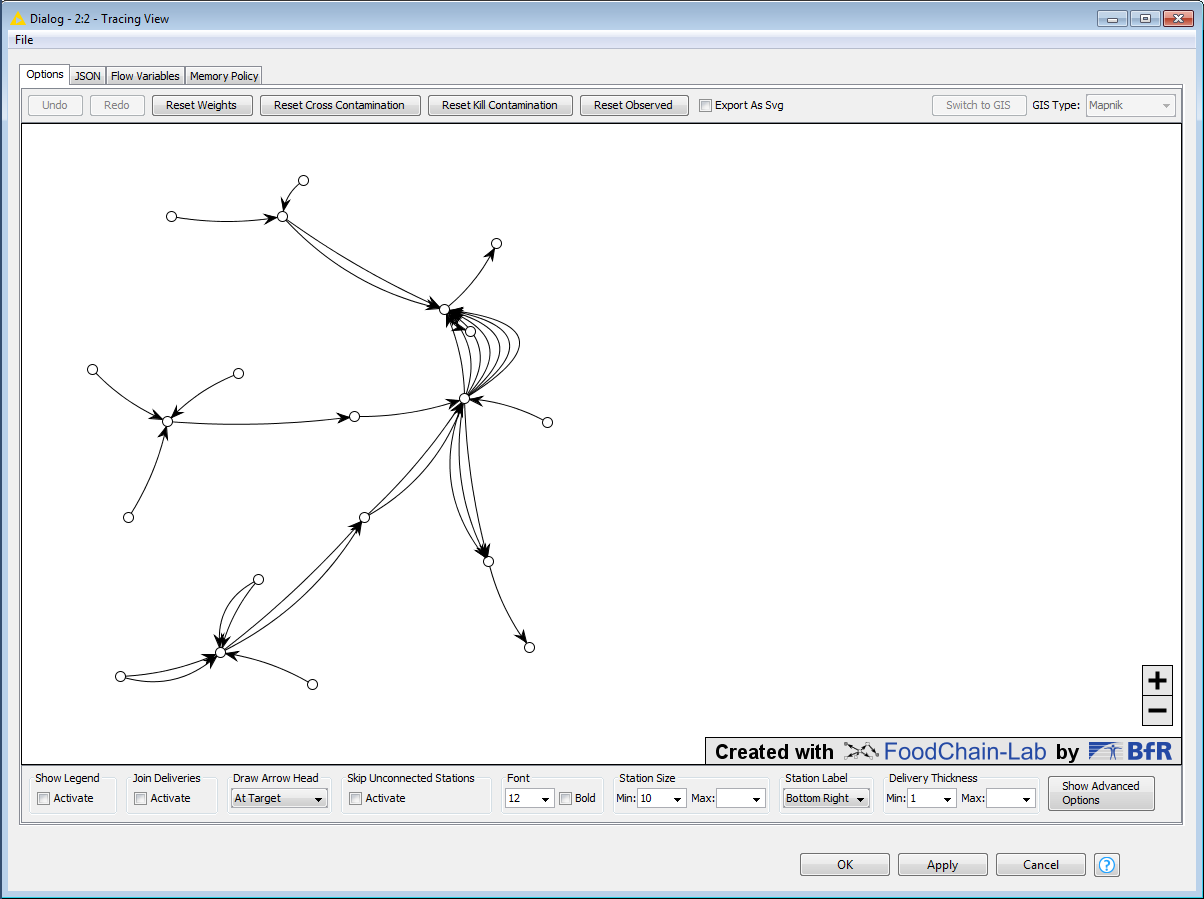
\includegraphics[height=0.6\textheight]{15.png}
	\end{center}
	\begin{itemize}
		\item Double click on the \textbf{Tracing View} node to configure it.
		\item You can see a network of stations (circles) and deliveries (arrows).
		\item In this network of a fictitious foodborne disease outbeak a contaminated product could be found in three supermarkets. We want to mark them as outbreak stations.
	\end{itemize}
\end{frame}

\section{16}
\begin{frame}
	\begin{center}
  		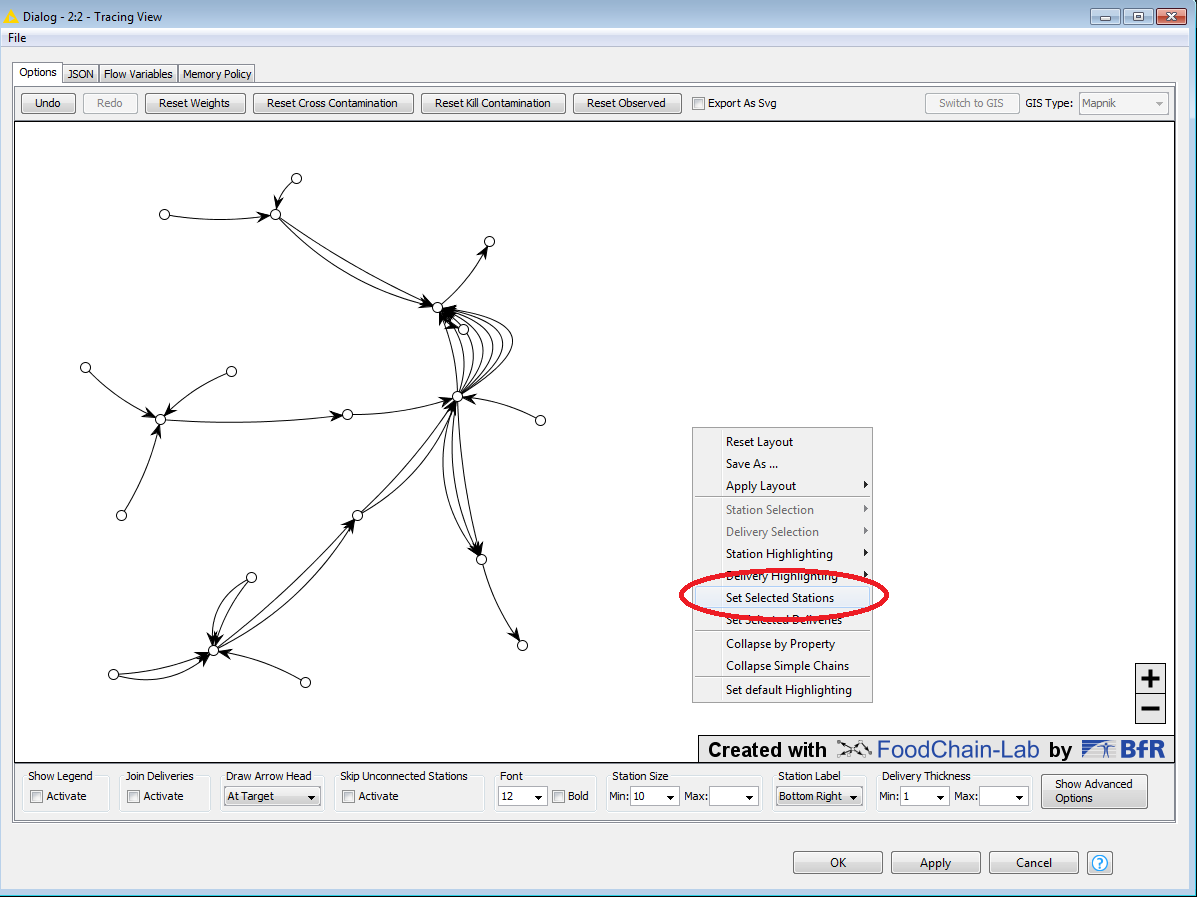
\includegraphics[height=0.6\textheight]{16.png}
	\end{center}
	\begin{itemize}
		\item To do so, right click somewhere into the empty space and choose \textbf{Set Selected Stations}.
	\end{itemize}
\end{frame}

\section{17}
\begin{frame}
	\begin{center}
  		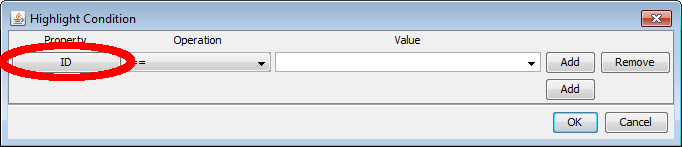
\includegraphics[width=0.9\textwidth]{17.png}
	\end{center}
	\begin{itemize}
		\item In this dialog you can specify which stations should be selected.
		\item Press the button in the red circle to set the \textbf{Property}.
	\end{itemize}
\end{frame}

\section{18}
\begin{frame}
	\begin{center}
  		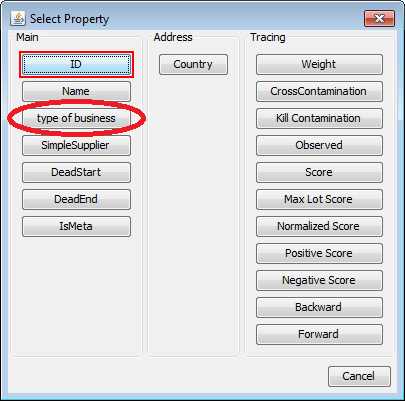
\includegraphics[width=0.4\textwidth]{18.png}
	\end{center}
	\begin{itemize}
		\item Select ``type of business''.
		\item Typical types of business are ``primary producer'', ``supplier'' and ``manufacturer'', for example.
	\end{itemize}
\end{frame}

\section{19}
\begin{frame}
	\begin{center}
  		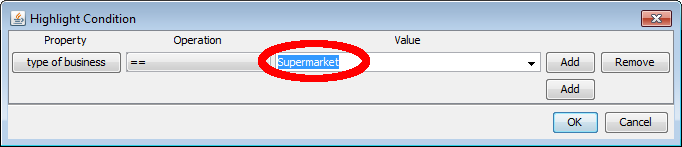
\includegraphics[width=0.7\textwidth]{19.png}
	\end{center}
	\begin{itemize}
		\item We only want to select supermarkets, since this is where contaminated products were found.
		\item Set \textbf{Value} to ``Supermarket'' and press \textbf{OK}. You can either click the small dropdown button on the right of the value field and select an entry or you type ``Supermarket'' into the white value field.
		\item Click \textbf{OK}.
	\end{itemize}
\end{frame}

\section{20}
\begin{frame}
	\begin{center}
  		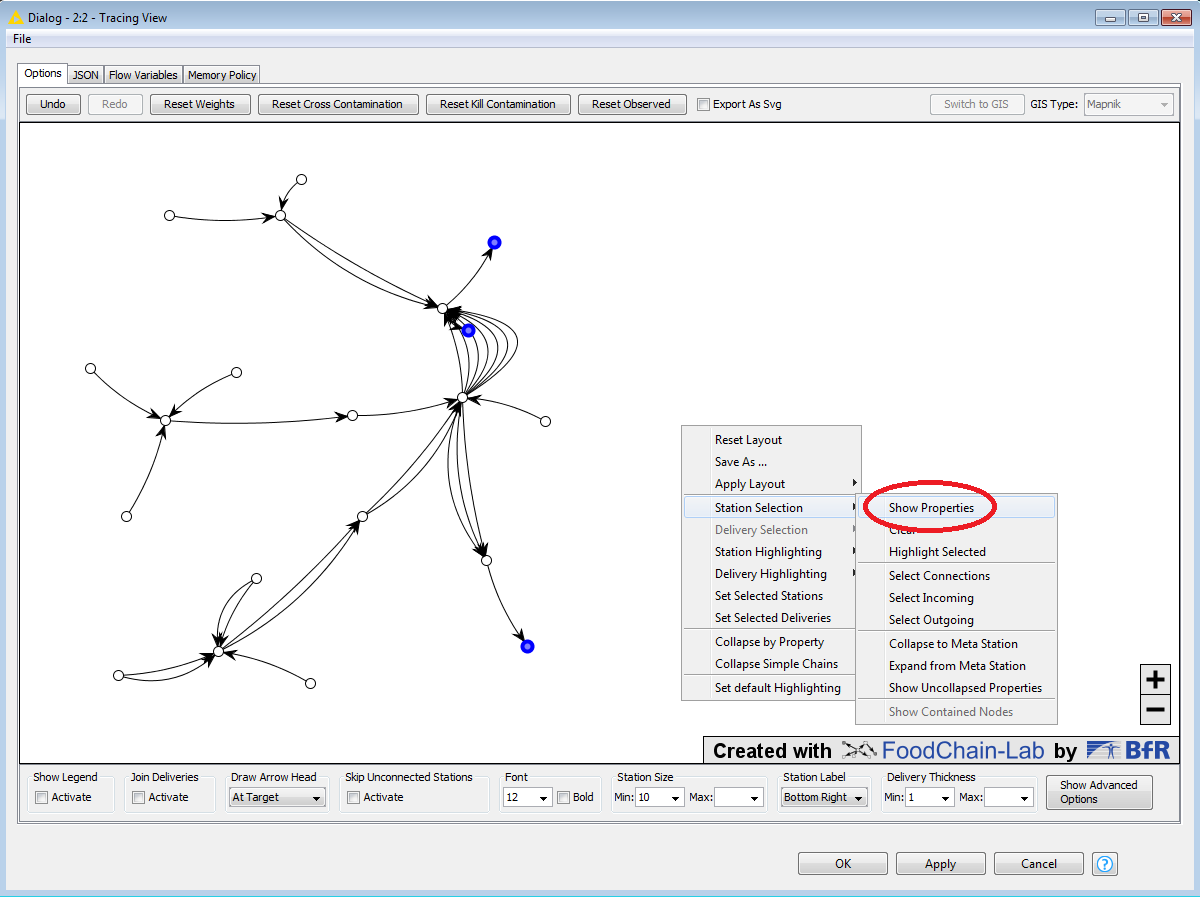
\includegraphics[height=0.6\textheight]{20.png}
	\end{center}
	\begin{itemize}
		\item Now, three stations are selected (blue circles).
		\item Right click somewhere into the empty space and choose \textbf{Station Selection} and \textbf{Show Properties}.
	\end{itemize}
\leftskip2.1em{\small Note: If you accidentally click with the left mouse button, you deselect all selected stations. Please go one step back to select the three supermarkets again.\par}
\end{frame}

\section{21}
\begin{frame}
	\begin{center}
  		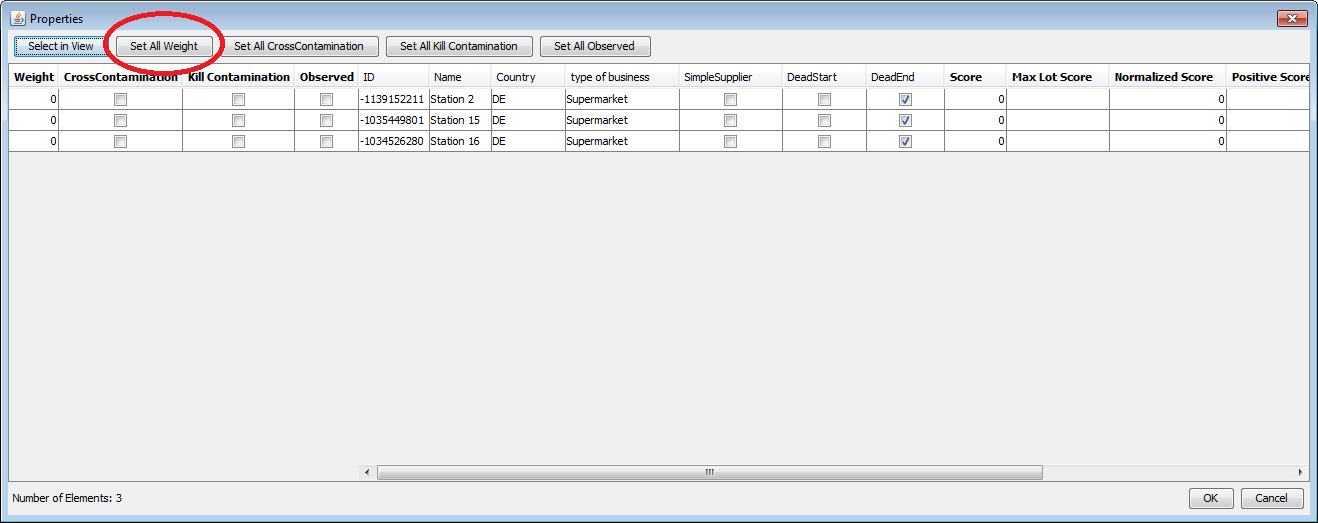
\includegraphics[width=0.9\columnwidth]{21.png}
	\end{center}
	\begin{itemize}
		\item A window pops up and you see the properties of the three selected supermarkets.
		\item Click \textbf{Set All Weight}.
	\end{itemize}
\end{frame}

\section{22}
\begin{frame}
	\begin{center}
			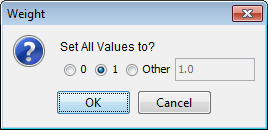
\includegraphics[width=0.5\columnwidth]{22.png}
	\end{center}
	\begin{itemize}
		\item By setting the weight to ``1'' you mark all supermarkets as outbreak stations. Here, ``1'' is already selected and you simply need to click \textbf{OK}.
	\end{itemize}
\end{frame}

\section{23}
\begin{frame}
	\begin{center}
			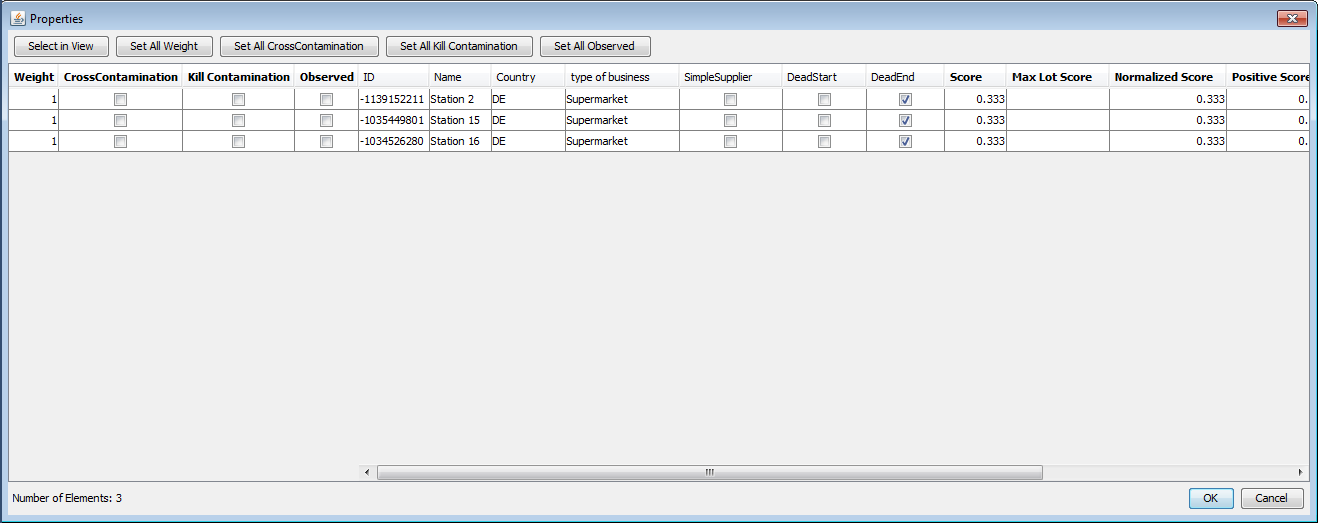
\includegraphics[width=0.9\columnwidth]{23.png}
	\end{center}
	\begin{itemize}
		\item All three supermarkets have a weight of ``1'' now.
		\item Another way to set the weight would be to click directly into one of the cells of the weight column and to type in the weight for each station individually.
		\item Click \textbf{OK}.
	\end{itemize}
\end{frame}

\section{24}
\begin{frame}
	\begin{center}
			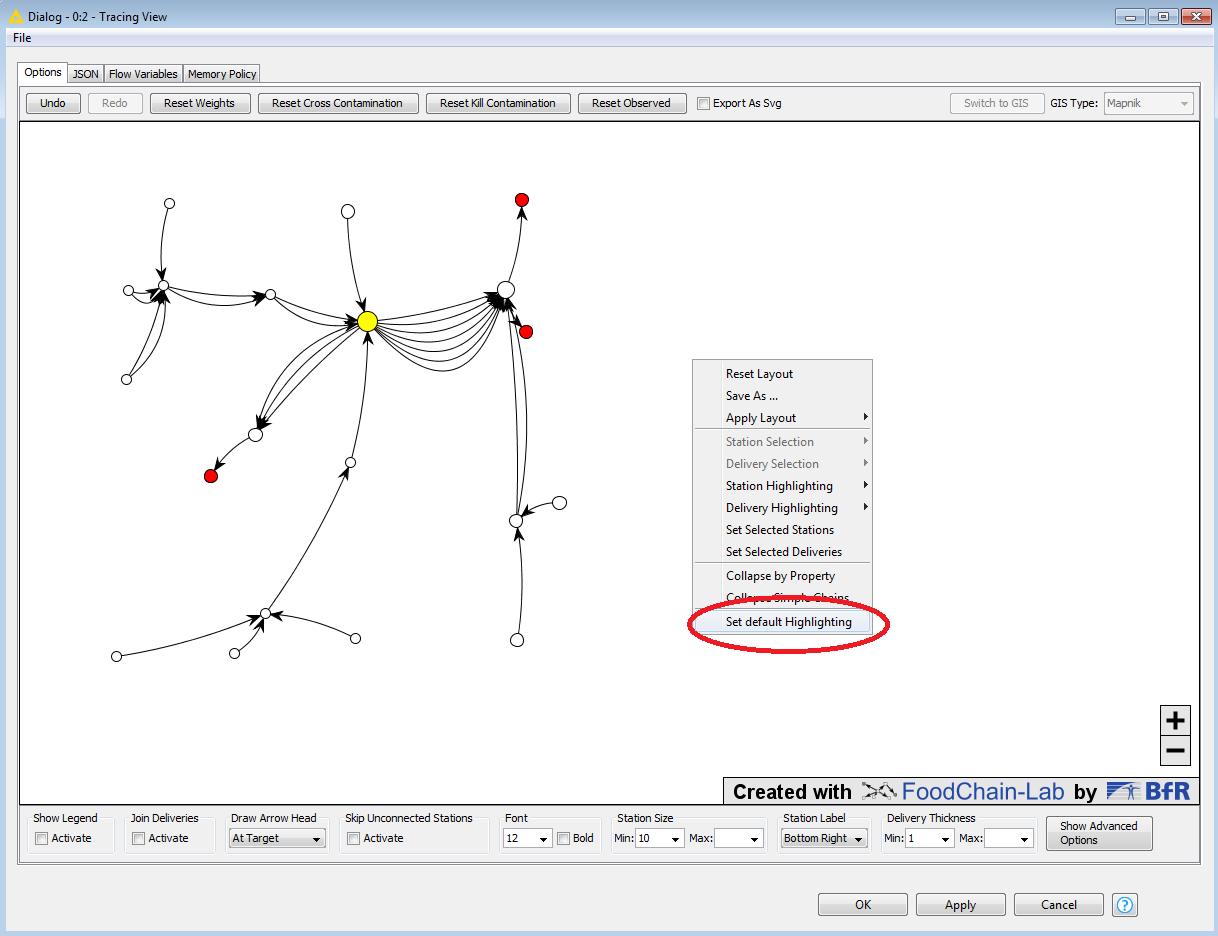
\includegraphics[height=0.6\textheight]{24.png}
	\end{center}
	\begin{itemize}
		\item Left click into the white network area to deselect highlighted stations (and deliveries) and you will see... nothing new.
		\item To get the image you see above, open the context menu (right click) and click \textbf{Set default Highlighting}.
	\end{itemize}
\end{frame}

\section{25}
\begin{frame}
	\begin{center}
			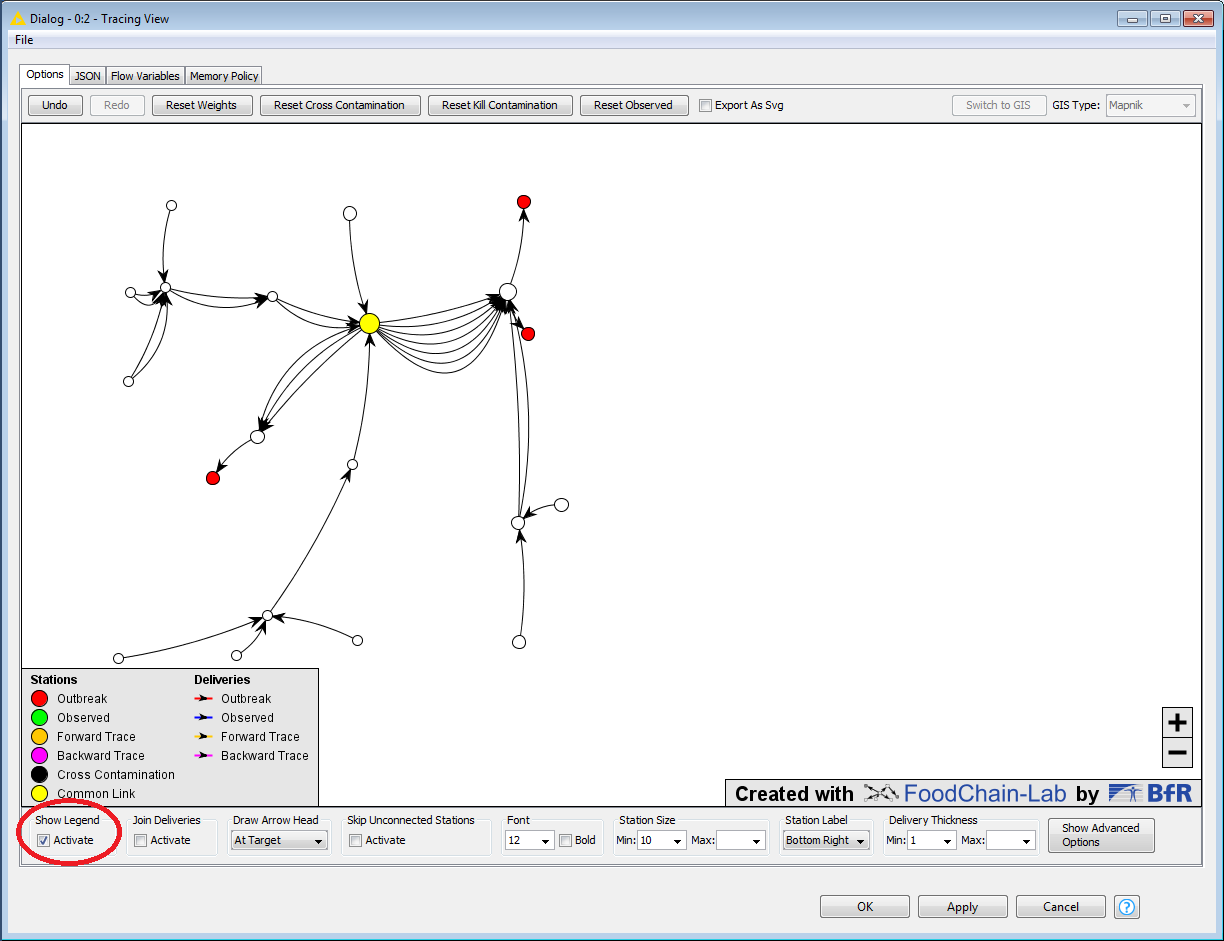
\includegraphics[height=0.6\textheight]{25.png}
	\end{center}
	\begin{itemize}
		\item Tick the box below \textbf{Show Legend} to display the legend. Here it is shown what the colours and symbols in the graph mean.
		\item So, the outbreak stations are red and the common link is yellow. The common link is a station which is connected (via identical ingredient lots or products thereof) with two or more outbreak stations in the same food chain.
	\end{itemize}
\end{frame}

\section{26}
\begin{frame}
	\begin{center}
  		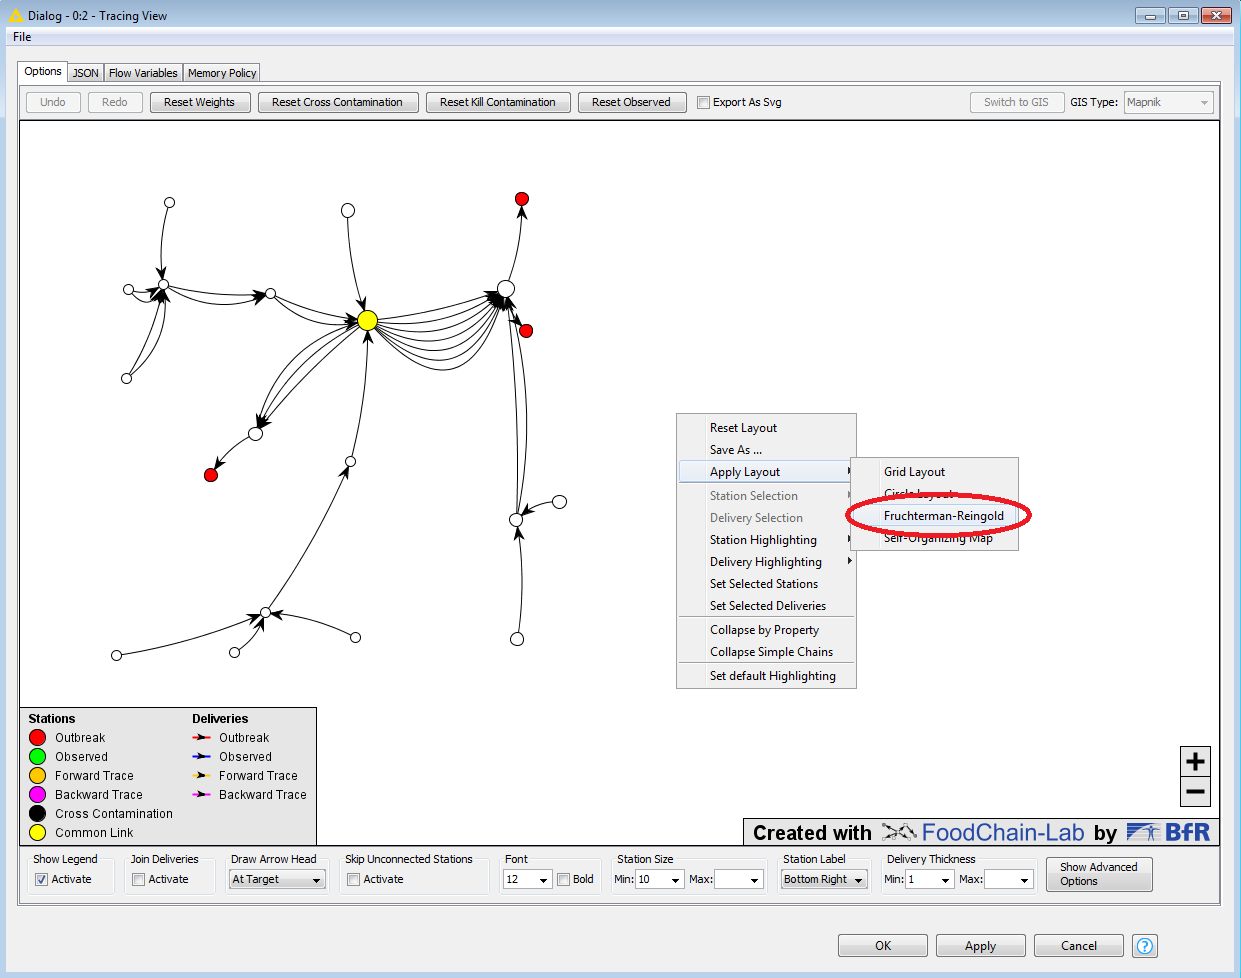
\includegraphics[height=0.6\textheight]{26.png}
	\end{center}
	\begin{itemize}
		\item To arrange the network in a better way right click in the graph and select \textbf{Apply Layout} and choose a layout, for example \textbf{Fruchterman-Reingold}.
	\end{itemize}
\end{frame}

\section{27}
\begin{frame}
	\begin{center}
  		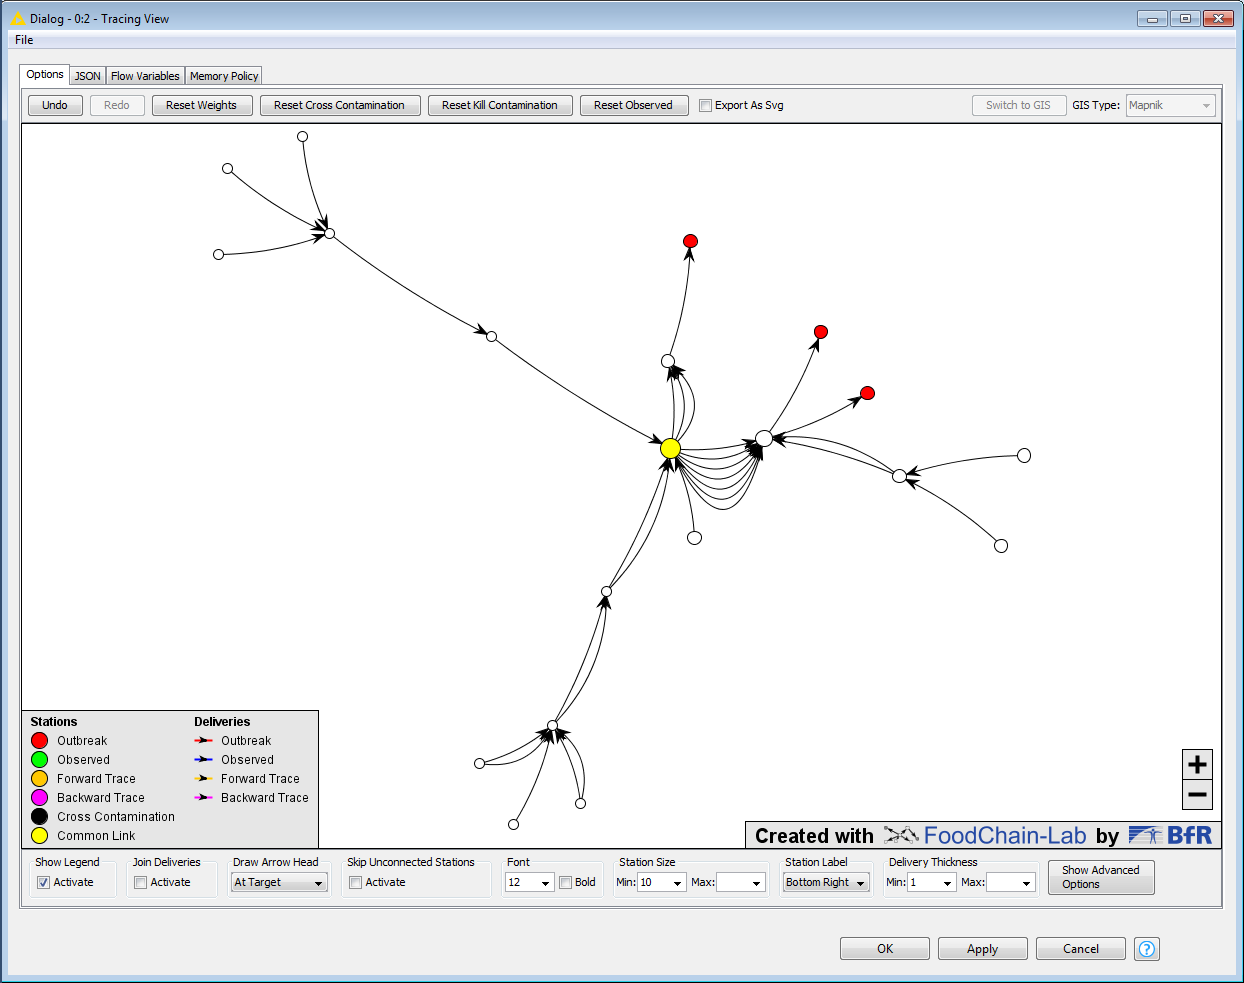
\includegraphics[height=0.6\textheight]{27.png}
	\end{center}
	\begin{itemize}
		\item This layout process is not deterministic. That means you will get a different result each time.
		\item You can apply the layout again, if you are not satisfied with the current result.
		\item You can also apply a layout for certain stations only:  Therefore you have to select the stations you want to be layouted and apply the layout again.
	\end{itemize}
\end{frame}

\section{28}
\begin{frame}
	\begin{center}
  		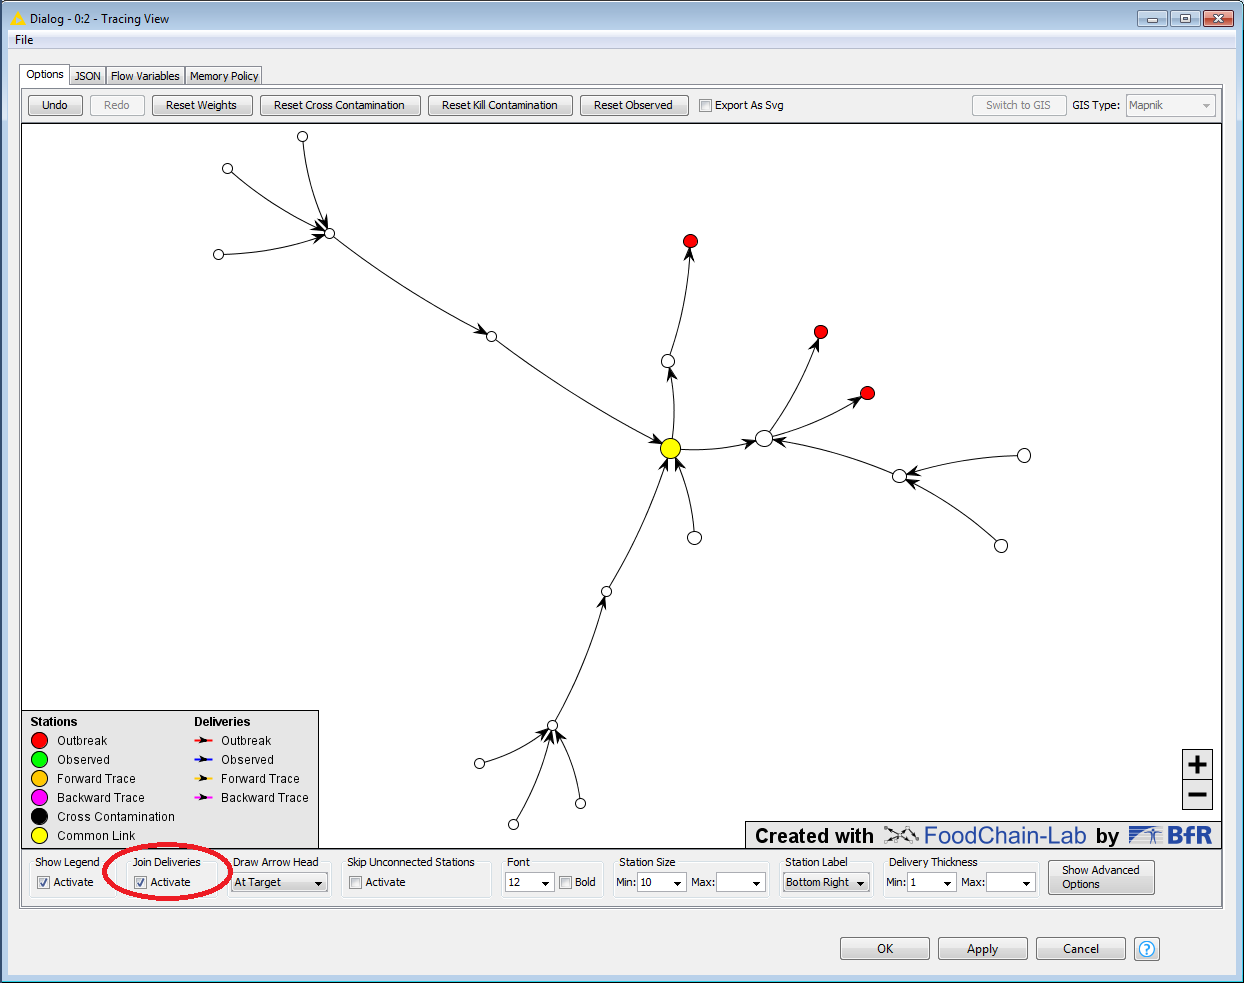
\includegraphics[height=0.6\textheight]{28.png}
	\end{center}
	\begin{itemize}
		\item You can activate \textbf{Join Deliveries} to simplify the graph. Deliveries with the same supplier and recipient are joined now.
		\item This option is especially useful in networks with many deliveries.
	\end{itemize}
\end{frame}

\section{29}
\begin{frame}
	\begin{center}
  		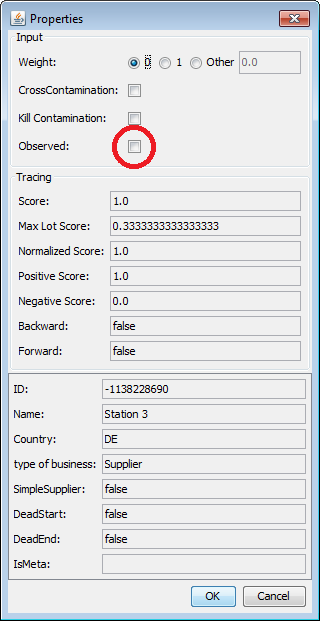
\includegraphics[height=0.6\textheight]{29.png}
	\end{center}
	\begin{itemize}
		\item Double click on the station marked as ``common link''.
		\item The dialog shown above will pop up, showing all attributes of the station.
		\item Select \textbf{Observed} and click \textbf{OK}.
	\end{itemize}
\end{frame}

\section{30}
\begin{frame}
	\begin{center}
  		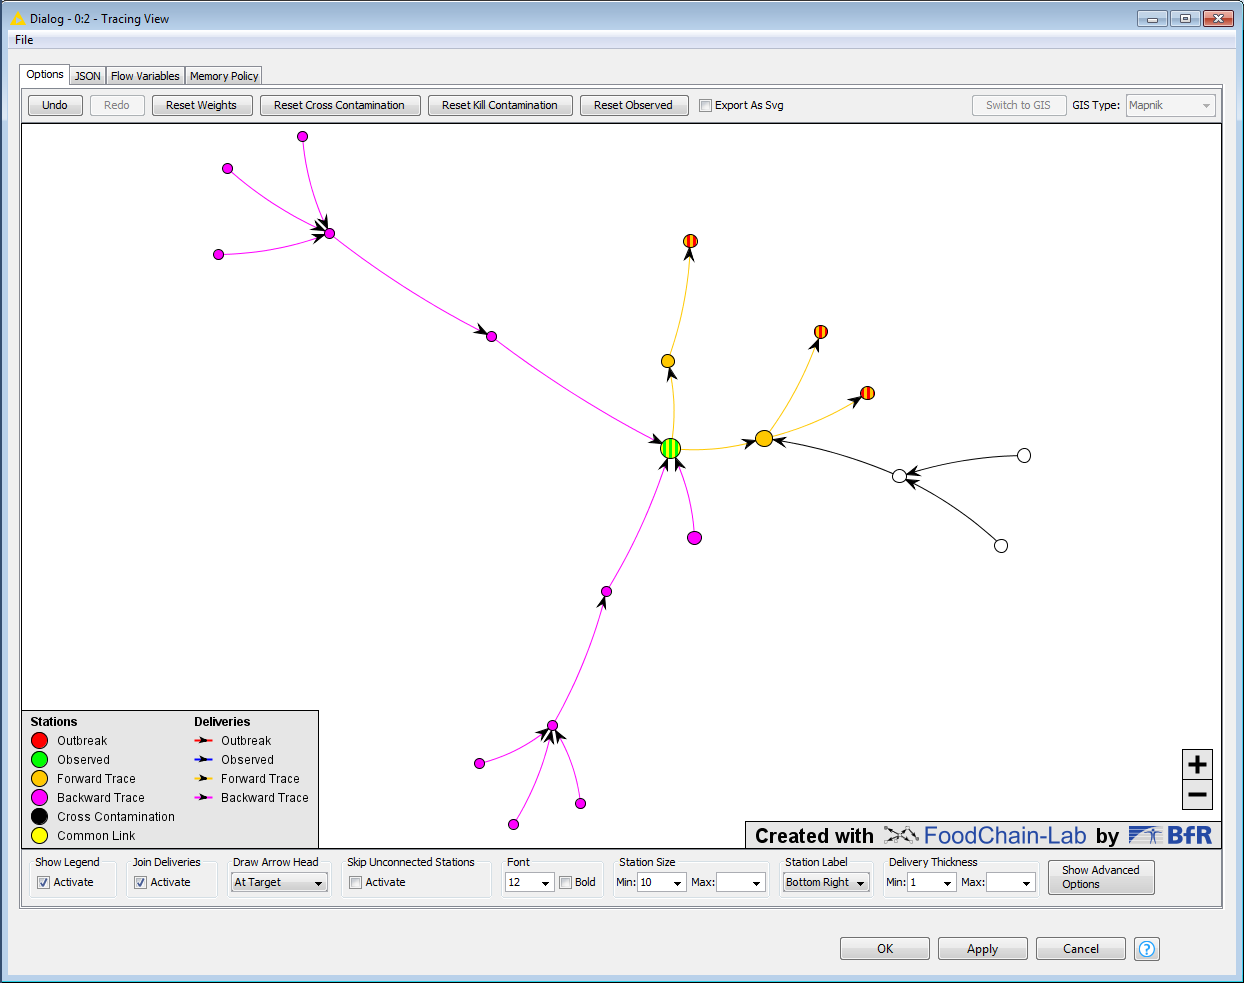
\includegraphics[height=0.6\textheight]{30.png}
	\end{center}
	\begin{itemize}
		\item All stations / deliveries of the forward trace are orange-colored and the ones of the backward trace are shown in purple.
		\item We will go into detail on this in the tutorial \textcolor{blue}{\underline{\href{https://foodrisklabs.bfr.bund.de/en_tracing/}{``Tracing''}}}.
	\end{itemize}
\end{frame}

\end{document}
